\chapter{其它形式的优化手段}

\section{View 的异步创建}

Feed 流本身并不局限于视频场景。如微信、今日头条、美团等应用的 Feed 流更多程度上是图文形式、非粘性滑动、具有大量内容的 RecyclerView。在这些场景下,预渲染的思路本身就不适合引入,因为这些场景下屏幕上同时有非常多的卡片,并且由于非粘性滑动,用户的每一次滑动都不是准确的定位到一个特定的卡片。因此,对于这些场景,更多的优化手段是让首次刷新更加迅速、让卡片创建的耗时尽可能降低等等。本文中主要采用的优化手段为将卡片进行异步创建(Inflate)。

在正常的 RecyclerView 创建卡片时,都是通过 Adapter 的回调实现卡片创建的逻辑。在内部通常会使用布局加载器 LayoutInflater 来通过 XML 文件加载 View。这种方式最耗时的任务就是对于 XML 文件的解析,并根据文件中的 View 层级创建出 View 实例的操作。如果将这部分流程提前进行,在用到的时候直接从缓存池中取用,就能够极大程度地减少 View 创建的耗时。谷歌官方已经提供了将 View 进行异步创建的组件 —— AsyncLayoutInflater。该组件内部拥有一个异步线程以运行业务方提交的 View 加载任务。但是异步创建 View 的难点并不是使用组件进行加载,而是找到加载的时机和用于保存加载出的 View 的缓存。

当 RecyclerView 被初始化时,内部还没有数据。需要等 Adapter 初始化完毕,并主动通知 RecyclerView 数据发生了变化之后,RecyclerView 才会进行相应的布局操作,并在这个过程中将子 View 初始化。在这个过程中,数据到达通常需要等待一段网络 IO 的时间。因此,在这个时间间隔内,我们可以用来进行 View 的异步创建。并且由于 RecyclerView 展示的子 View 的属性通常都是一致的,因此我们可以提前知晓 View 的具体类型,并通知异步的 AsyncLayoutInflater 进行加载;View 的缓存选用 SparseArray。因为 SparseArray 与 HashMap 有相似的结构,所以通过 View 的 id 去访问通常有更高的性能;同时如果需要大量的读写操作,SparseArray 也与队列等结构有相似的效率,比数组在移除、添加操作上有更高的效率。

\section{异步创建优化验证}

为了验证异步创建 View 优化的效果,搭建了一个类似新闻页面的 RecyclerView。此页面在首次刷新时会进行一次假的网络请求,在一段时间之后会返回一些新闻数据,同时用于 Adapter 进行数据绑定并通知 RecyclerView 进行布局。为了模拟 View 创建过程中的耗时行为,人为在子 View 的构造方法中引入耗时逻辑。在这个过程中,开启异步预加载和关闭预加载的情况下,可以明显感觉到有异步创建的时候加载的速度更快。为了进一步量化优化效果,设计了一个“秒开检测框架”:当 RecyclerView 首次刷新时,通过 ViewTreeObserver 的监听器捕获事件,并在回调方法中执行检测逻辑。

\begin{figure}
    \centering
    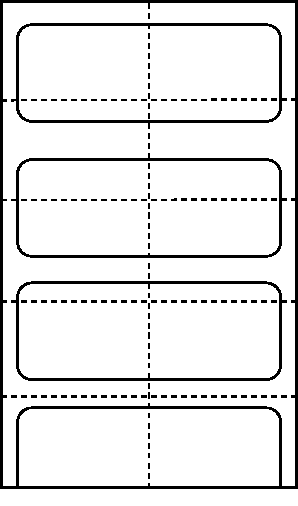
\includegraphics{assets/visibility-check.pdf}
    \caption{秒开检测框架的应用实例}
\end{figure}

\begin{figure}[H]
    \centering
    \begin{tikzpicture}
        \begin{axis}[
            ybar, % 使用柱状图样式
            width=13cm,
            scale=0.8,
            enlarge x limits={abs=0.5}, % 扩大 X 轴范围,确保边缘数据点完全显示
            ylabel={首刷时长(秒)}, % Y轴标签
            xlabel={缓存容量(个)},
            xmin=0, xmax=15, % X轴范围
            ymin=0, ymax=6, % Y轴范围
            xtick={0,1,...,15}, % X轴刻度
            ytick={0,0.5,...,6}, % Y轴刻度
            nodes near coords, % 在柱状图上显示具体数值
            nodes near coords align={vertical}, % 数值显示垂直方向
            every node near coord/.append style={font=\tiny, inner ysep=3pt} % 设置文字样式和距离
            ]
            \addplot[fill=blue!0] coordinates {
                (0, 5.17)(1, 5.17)(2, 5.33)(3, 4.51)(4, 4.44)(5, 4.3)
                (6, 4.06)(7, 3.83)(8, 3.59)(9, 3.38)(10, 3.16)(11, 3.52)
                (12, 3.51)(13, 3.93)(14, 4.33)(15, 4.74)
            }; % 添加柱状图数据,x=0,y=3.5
        \end{axis}
    \end{tikzpicture}
    \caption{首刷时长与缓存个数的关系}
\end{figure}



秒开框架的检测思路如图 8.1:将屏幕分成若干个目标区域,每个区域通过左上角顶点的坐标,以及区域的长和宽来唯一标识。当进行检测时,扫描检测范围内所有的 View,让业务方来决定有效区域的大小。这里的有效区域是指对用户来说有意义的区域大小。以文本类 TextView 来举例子,有效区域就是真实文本所覆盖的区域,不包括四周的留白。当有效区域和屏幕的目标区域的交集超过了一定阈值时,该目标区域被标记为有效;当所有(或大部分)的目标区域都被认为有效时,此时的时刻为页面首次刷新的时长,即首帧时长。该时长标志着应用加载的速度以及给用户带来的体感。时间越短表明对用户来说刷新的感知时间越短,体验越好。

当没有异步创建,以及有异步创建的情况下缓存容量逐渐增加的过程中,缓存容量与首帧时长的关系如图 8.2。可以发现,随着缓存容量不断扩大,能够提前预加载的 View 也不断变多,所以首刷时长会不断降低;但由于屏幕大小的限制,缓存数量也不是越多越好。当缓存个数超出屏幕能承载的最大 View 个数时,多出来的部分反而会让首次刷新变得更慢。所以我们需要针对具体的业务场景找到一个最佳的缓存池容量来实现最佳的首刷时长优化。